\section{Results}
All four algorithms are color-coded consistently throughout all six plots. The lines represent averages of 10 training runs. The error bars are based on the standard error at that point in time.

In Figure \ref{fig:10sized-nomem}, \ref{fig:10sized-100mem} and \ref{fig:10sized-1000mem} we see the three cases where the simulation consists of a grid of 10-by-10 and the algorithms are given no, 100 or 1000 episodes of demonstation data respectively.

Firstly, in Figure \ref{fig:10sized-nomem} we see that all algorithms struggle to beat the baseline algorithm. Only the Dueling Q-Networks is able to come near. It offers a greatly increased learning speed and is able to sustain a higher maximum performance level. The other three algorithm perform similarly to each other, but noticable worse than Dueling Q-Networks.

Secondly, in Figure \ref{fig:10sized-100mem} we see the performance of all algorithms converge. The Dueling Q-Networks which performed better than the others before, has now lost its edge and is now the worst performer. The performance of Q-Networks has greatly increased when fed $\pm 3500$ memories compared to none. It surpasses the baseline algorithm temporarily. SARSA and Dueling SARSA fly under the radar, but also increased their performances given more memories than before.

Lastly, in Figure \ref{fig:10sized-1000mem} we see each algorithm perform differently. The Q-Network loses performance compared to the previous configuration, but still performs better than when no memories were given. The Dueling Q-Network did not improve its performance with $\pm 35000$ memories and shows a peculiar peak near the 1000th episode. SARSA has increased its performance once again and now beats the baseline algorithm. The same holds for Dueling SARSA which outperforms SARSA. Dueling SARSA show the same, yet smaller, peculiar peak like Dueling Q-Networks. The two algorithms incorporating SARSA offer a noticeably lower standard error.

In Figure \ref{fig:14sized-nomem}, \ref{fig:14sized-100mem} and \ref{fig:14sized-1000mem} we see the three cases where the simulation has a grid size of 14-by-14 and the algorithms are given no, 100 or 1000 episodes of demonstation data.

Firstly, in Figure \ref{fig:14sized-nomem} we see results comparable to Figure \ref{fig:10sized-nomem}, however the performance difference of Dueling Q-Networks compared to the rest has decreased. The best performing algorithm here does not come close to the performance of the baseline.

Secondly, in Figure \ref{fig:14sized-100mem} we see results similar to Figure \ref{fig:10sized-100mem}, but no algorithm is able to beat the baseline like Q-Networks was able to before.

Lastly, in Figure \ref{fig:14sized-1000mem} we once again see results comparable to Figure \ref{fig:10sized-1000mem}, however only Dueling SARSA is now able to beat the baseline algorithm. SARSA is able to perform at the same level as the baseline in the end. The (Dueling) Q-Networks do not offer good performance, but Dueling Q-Networks does outperform Q-Networks.


\begin{figure}[h]
    \centering
    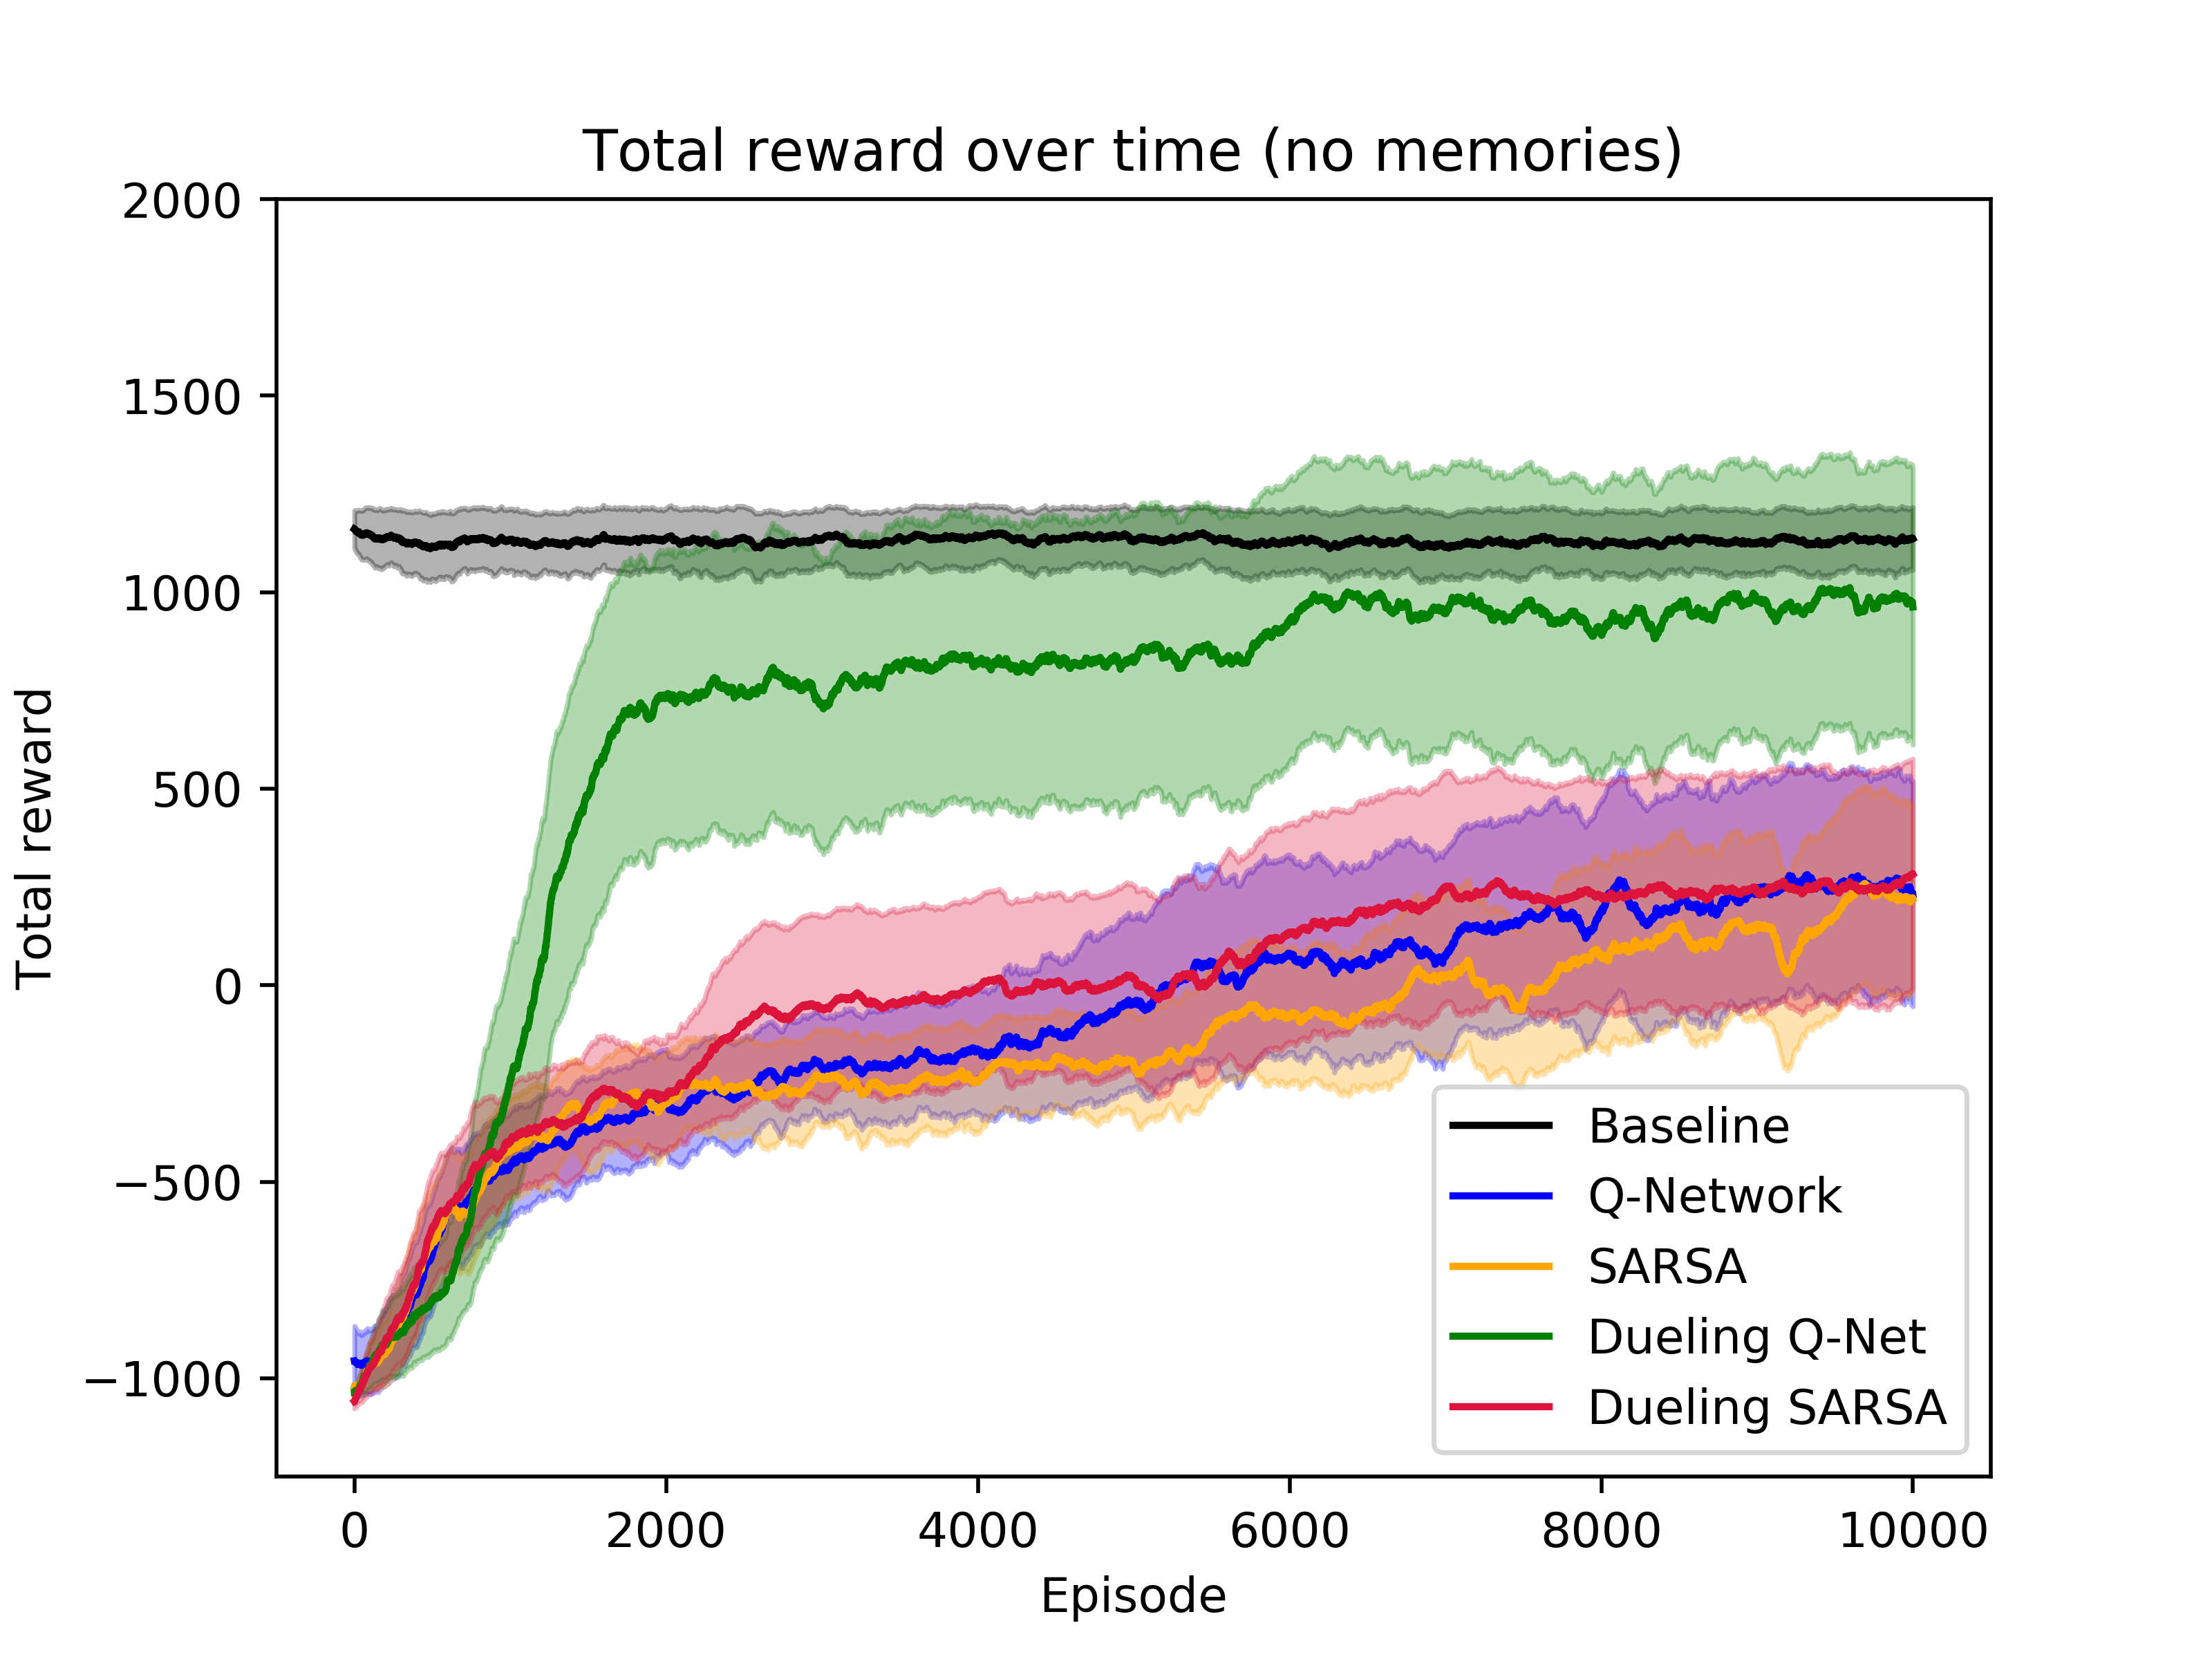
\includegraphics[width=\linewidth]{img/results/10-sized/total_rewards_0m-min.png}
    \caption{10-by-10 grid given no demonstation data.}
    \label{fig:10sized-nomem}
    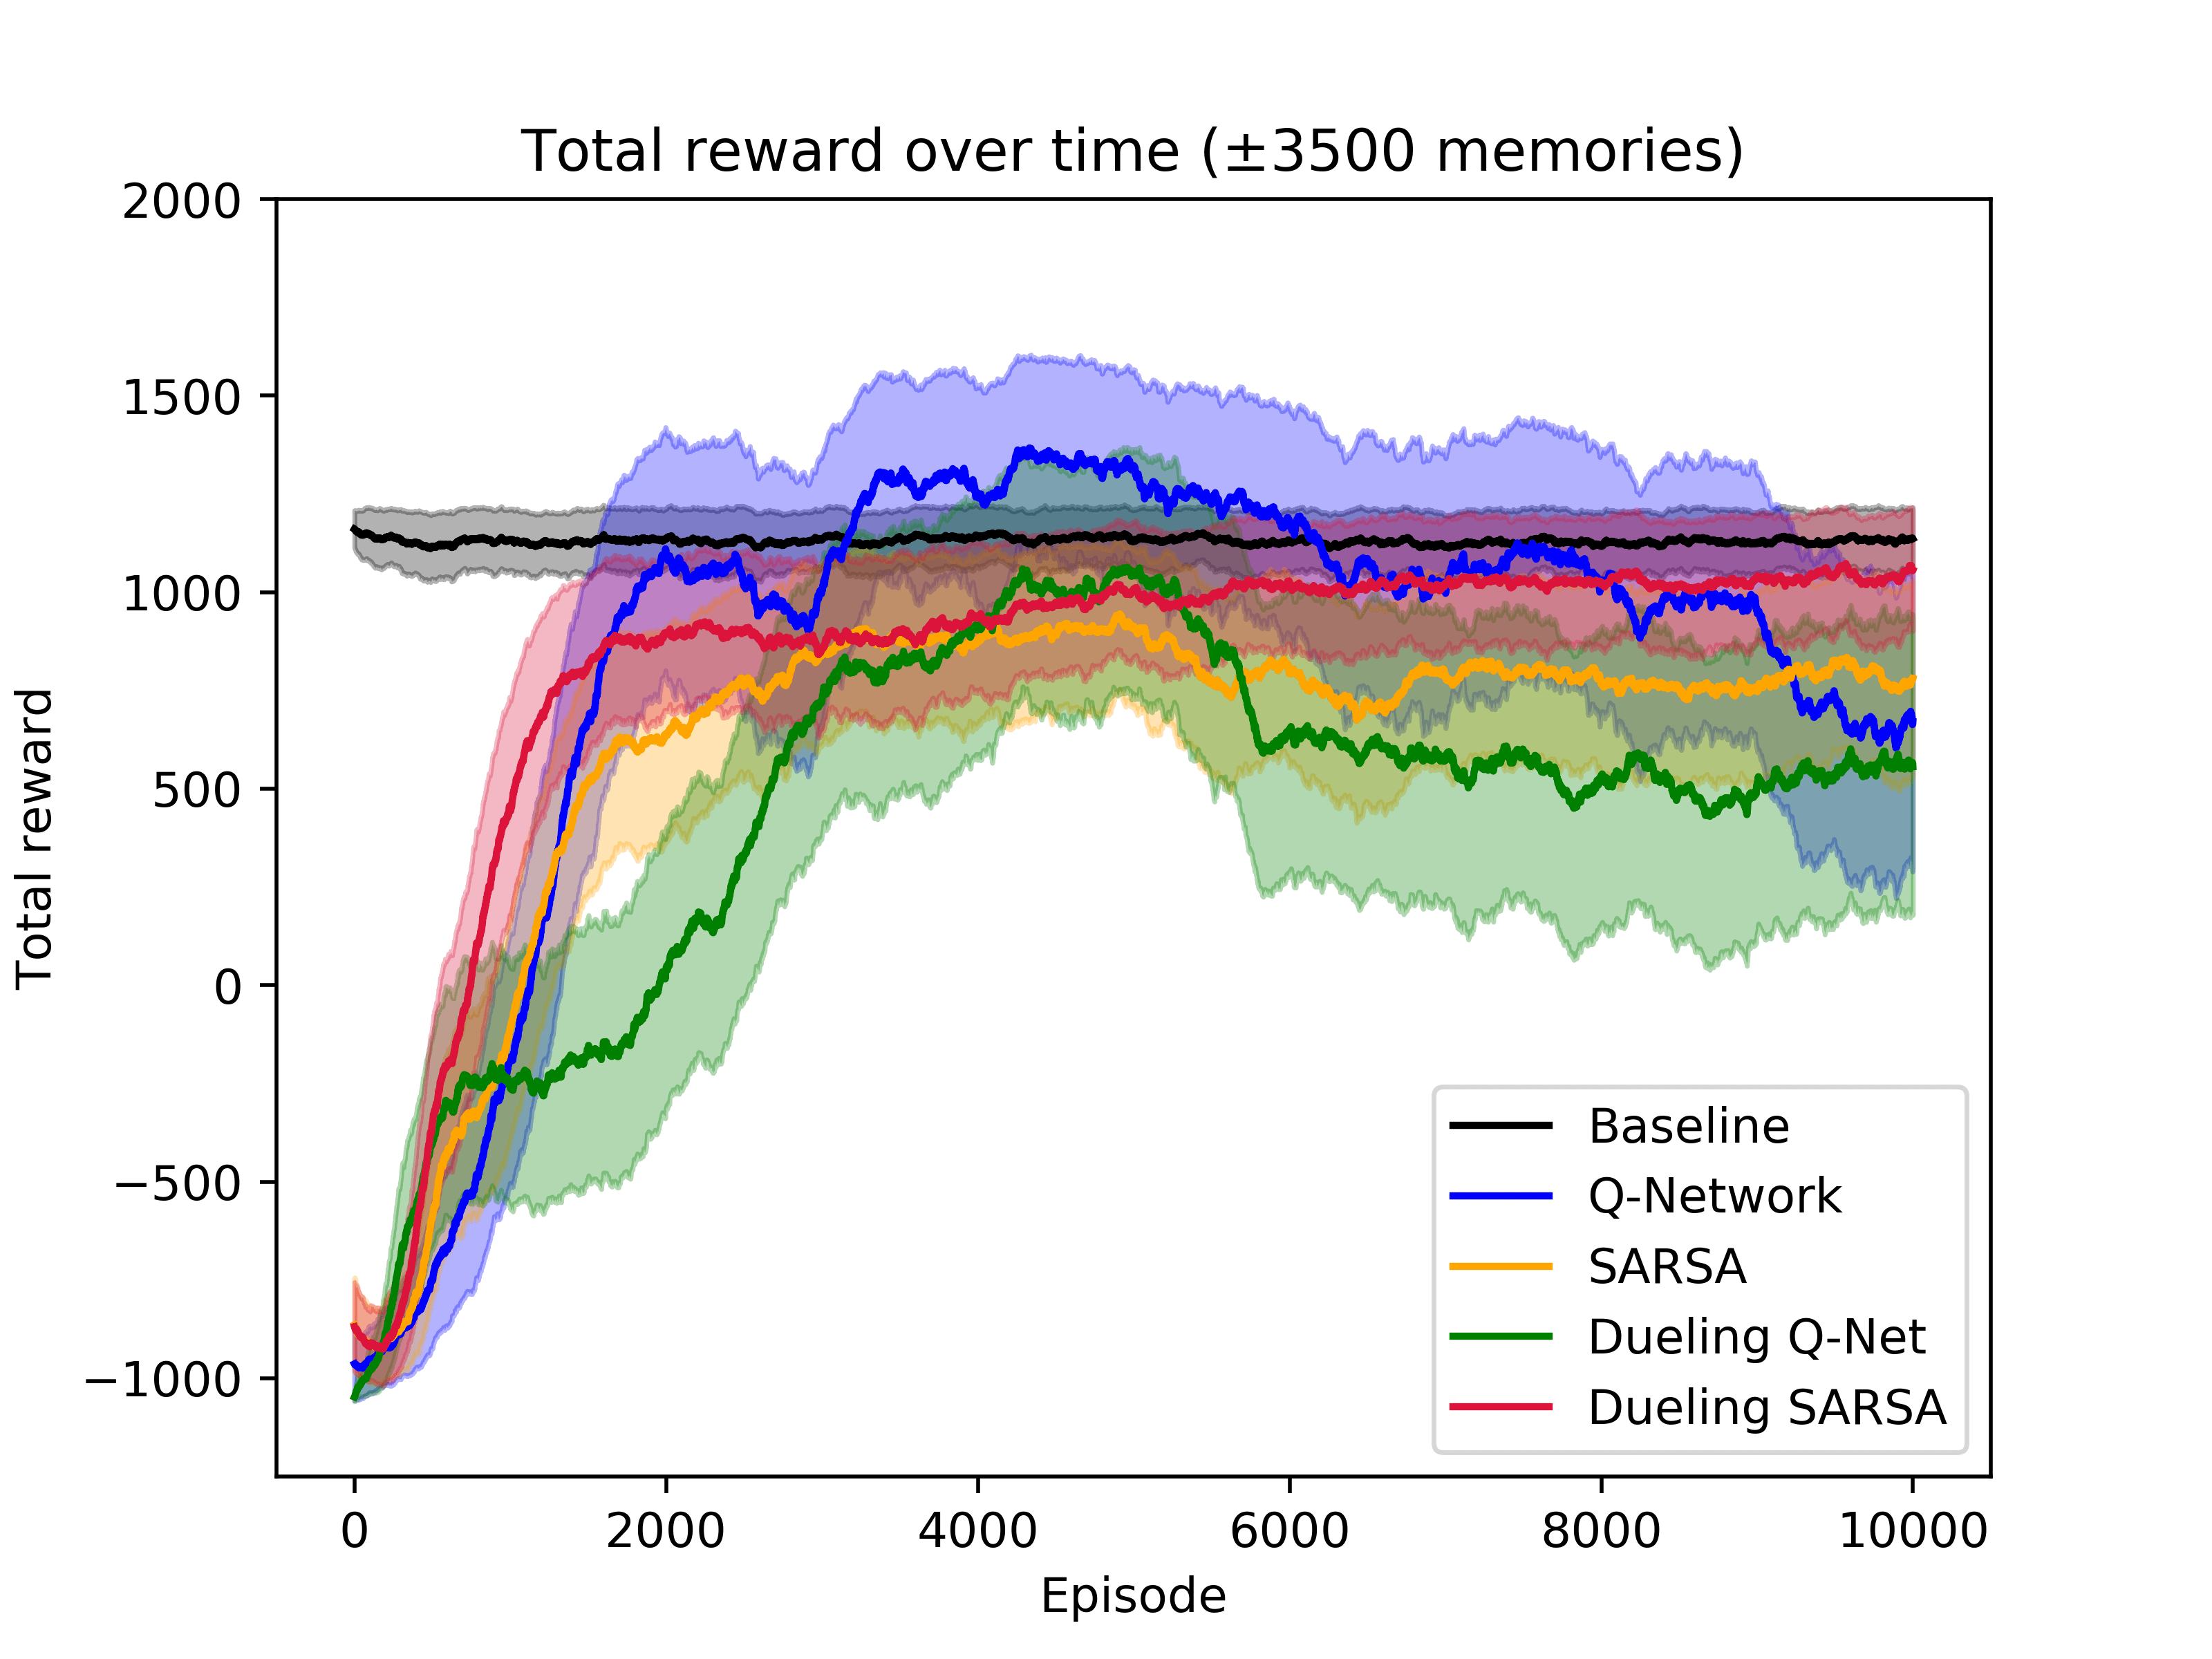
\includegraphics[width=\linewidth]{img/results/10-sized/total_rewards_100m-min.png}
    \caption{10-by-10 grid given 100 episodes of demonstation data.}
    \label{fig:10sized-100mem}
    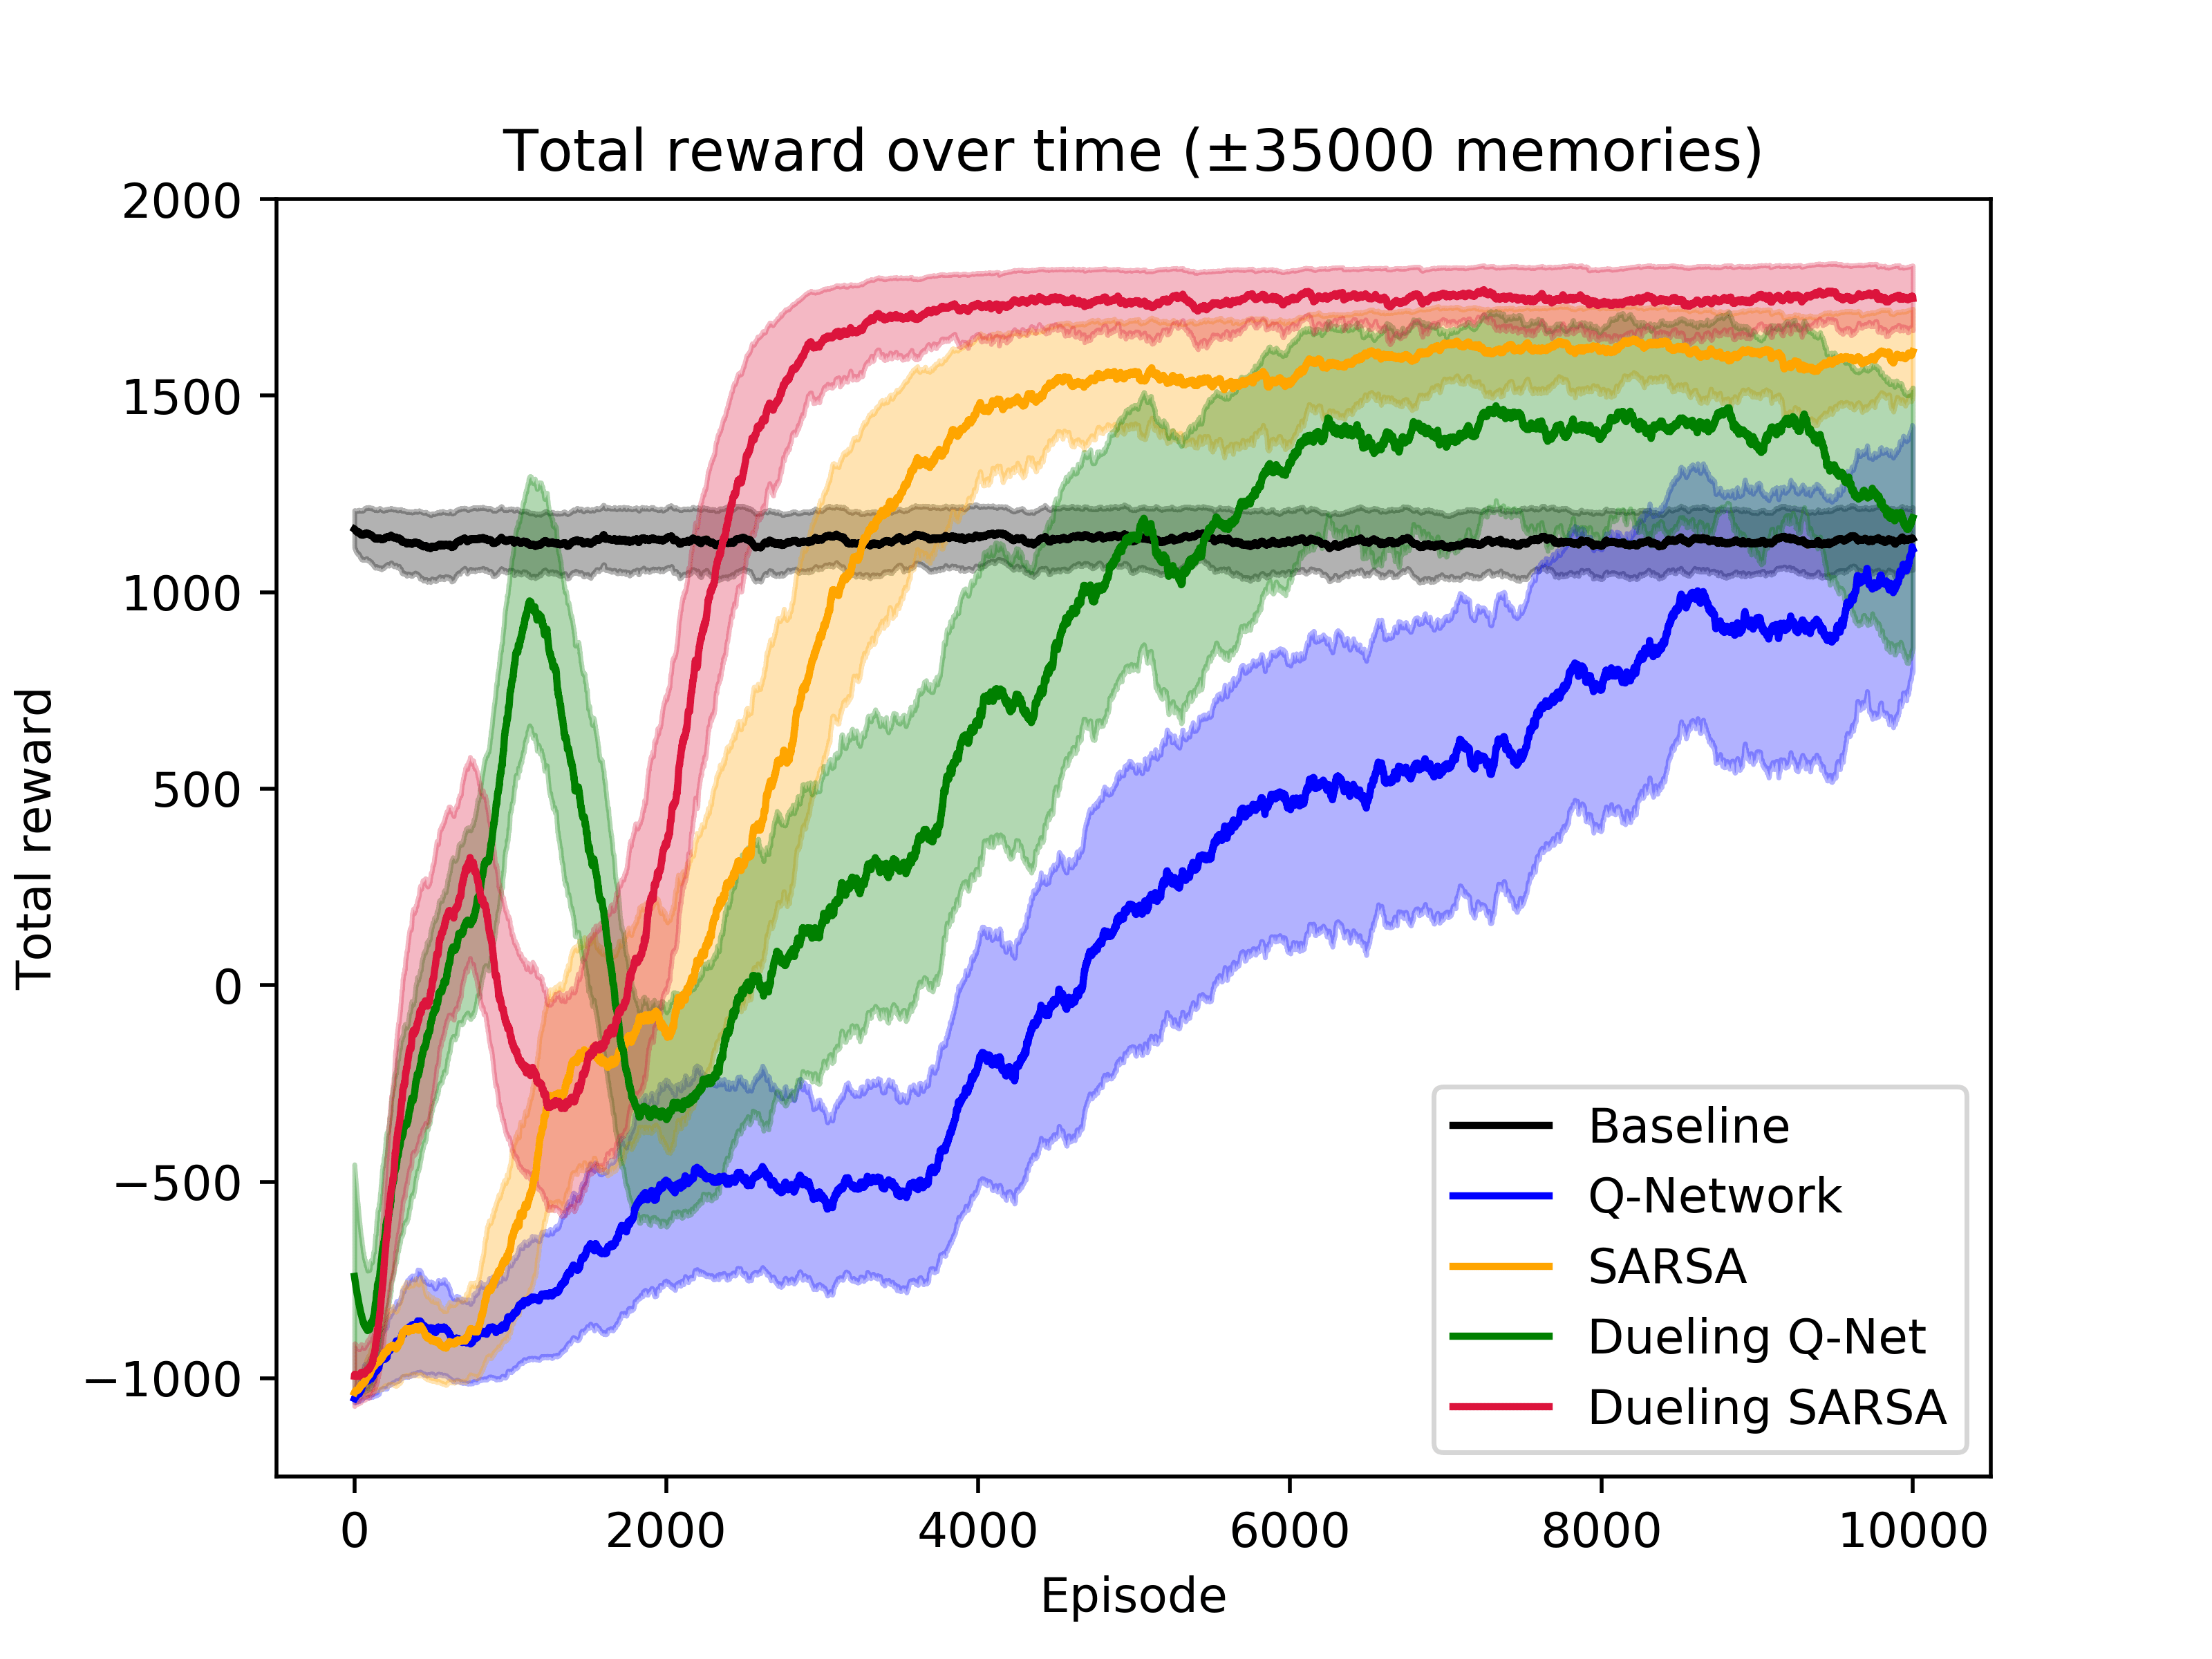
\includegraphics[width=\linewidth]{img/results/10-sized/total_rewards_1000m-min.png}
    \caption{10-by-10 grid given 1000 episodes of demonstation data.}
    \label{fig:10sized-1000mem}
\end{figure}
\begin{figure}[h]
    \centering
    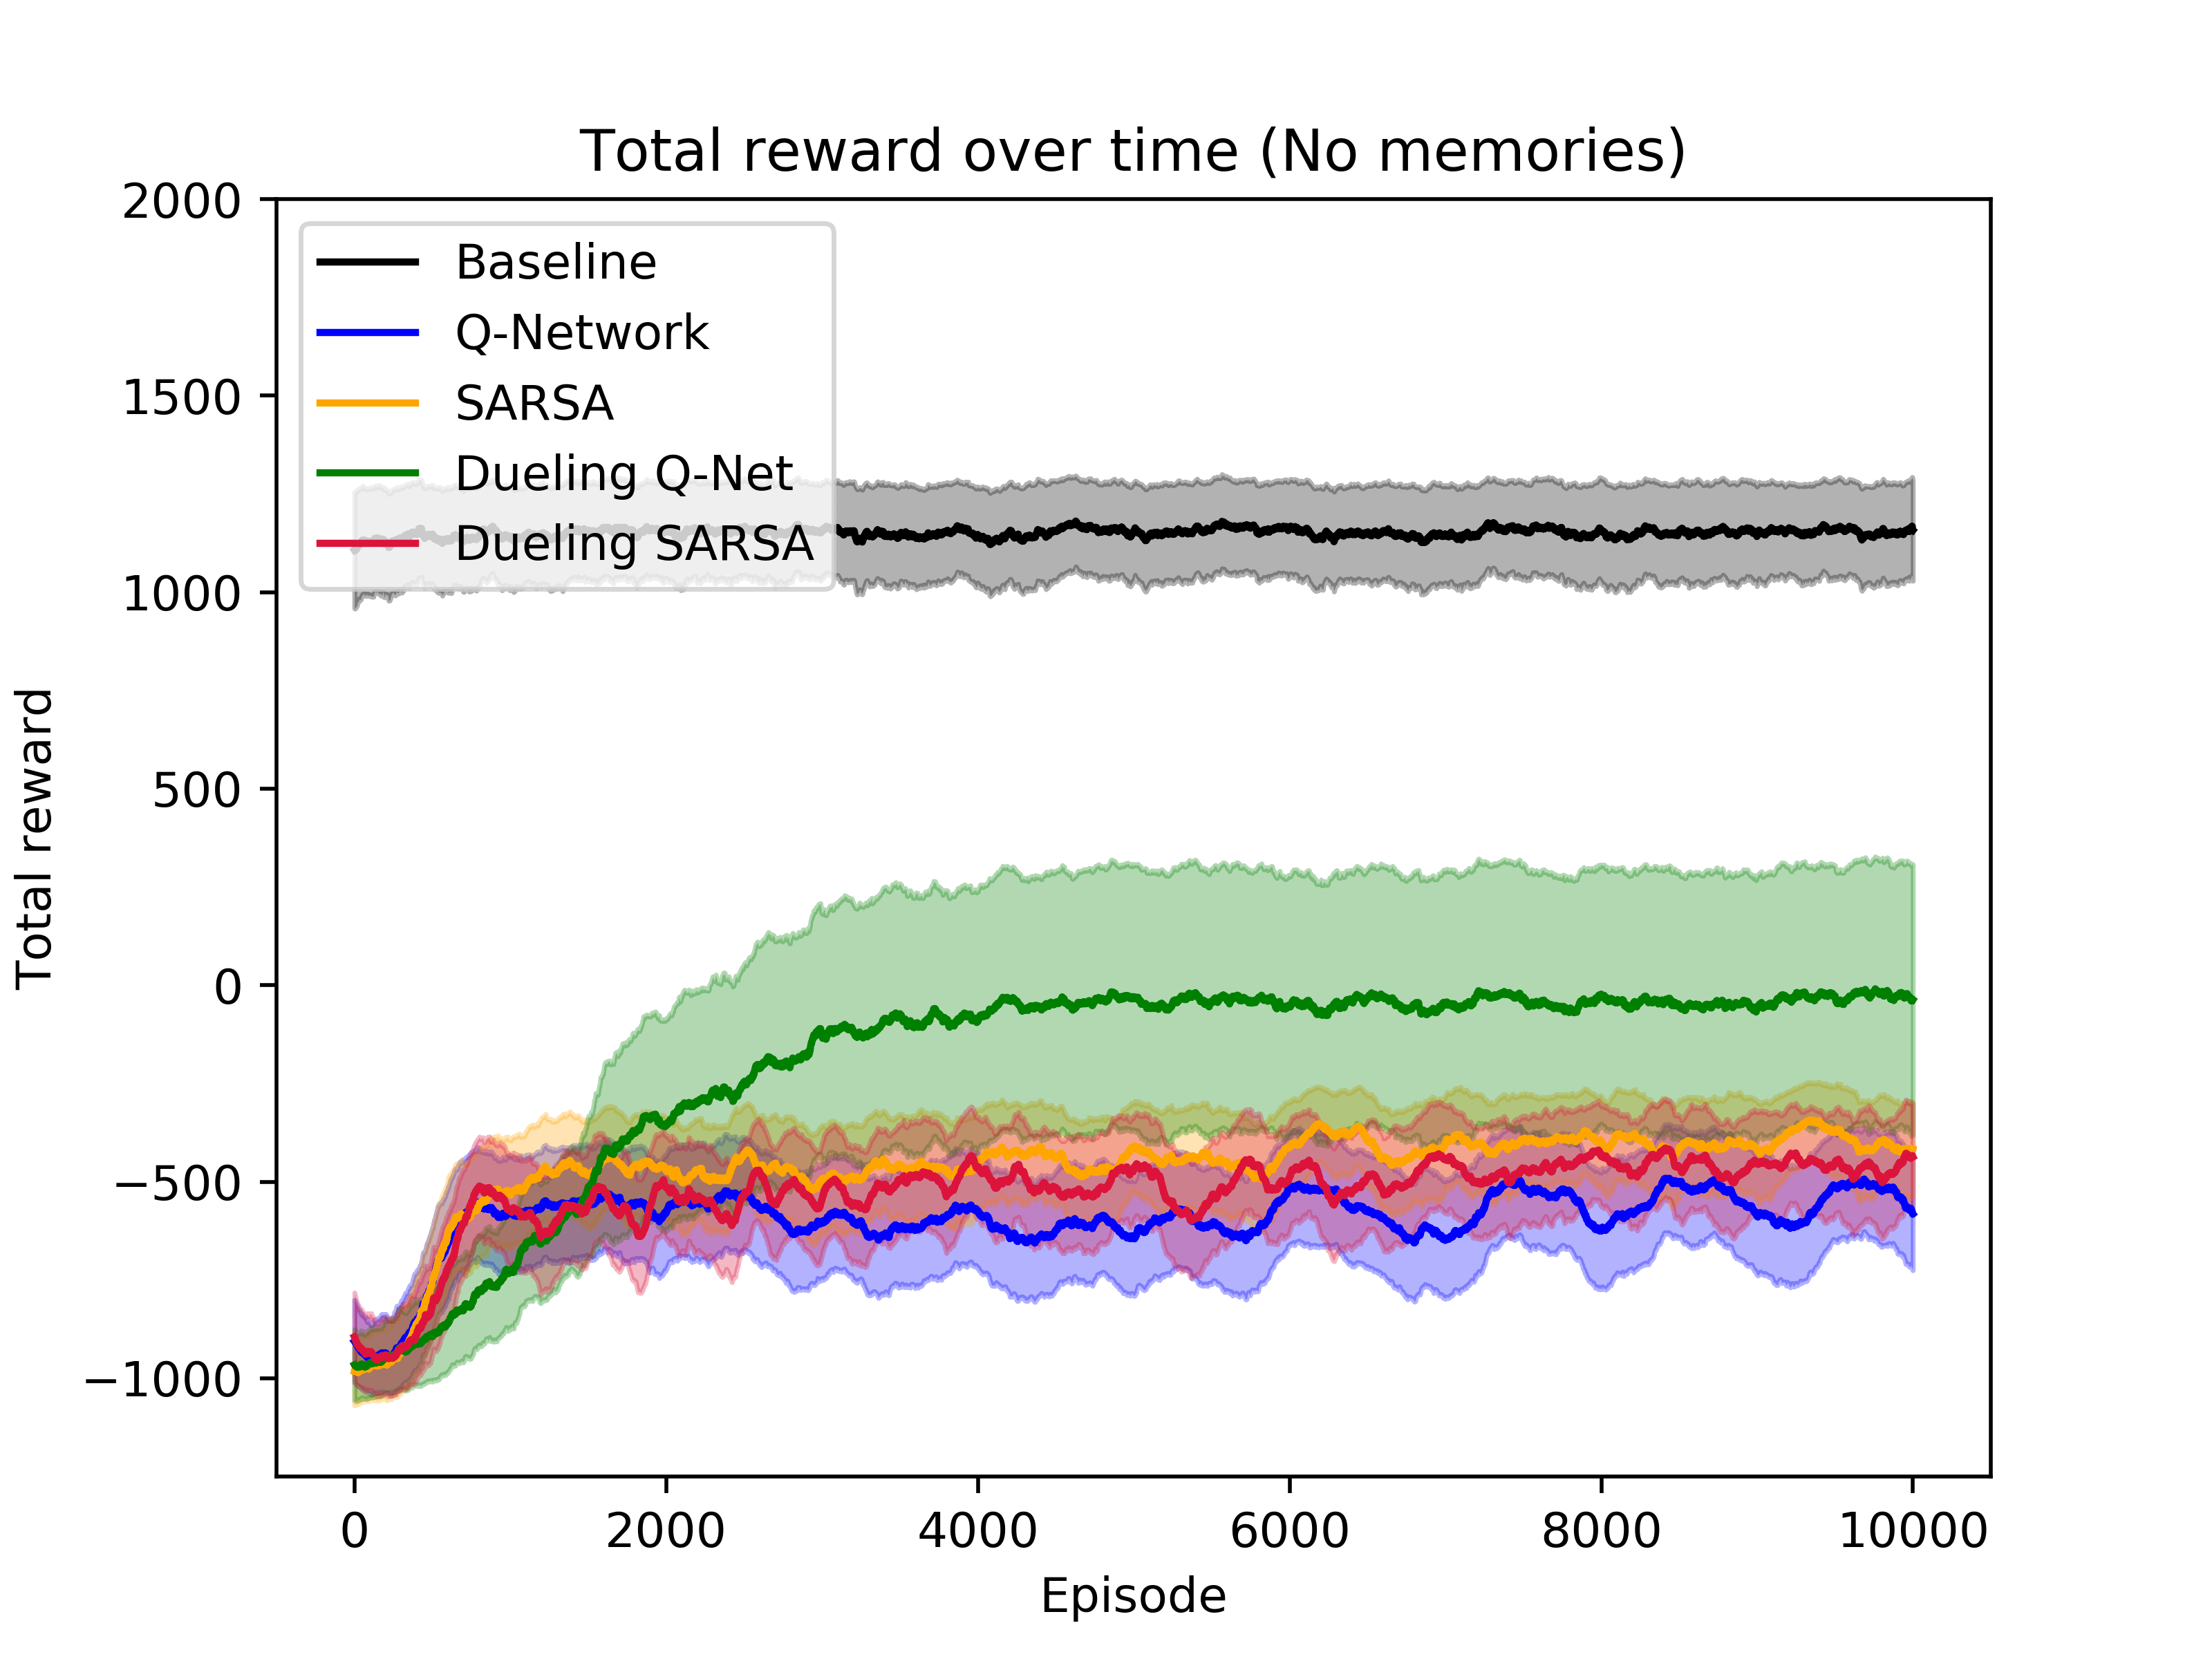
\includegraphics[width=\linewidth]{img/results/14-sized/total_rewards_0m-min.png}
    \caption{14-by-14 grid given no demonstation data.}
    \label{fig:14sized-nomem}
    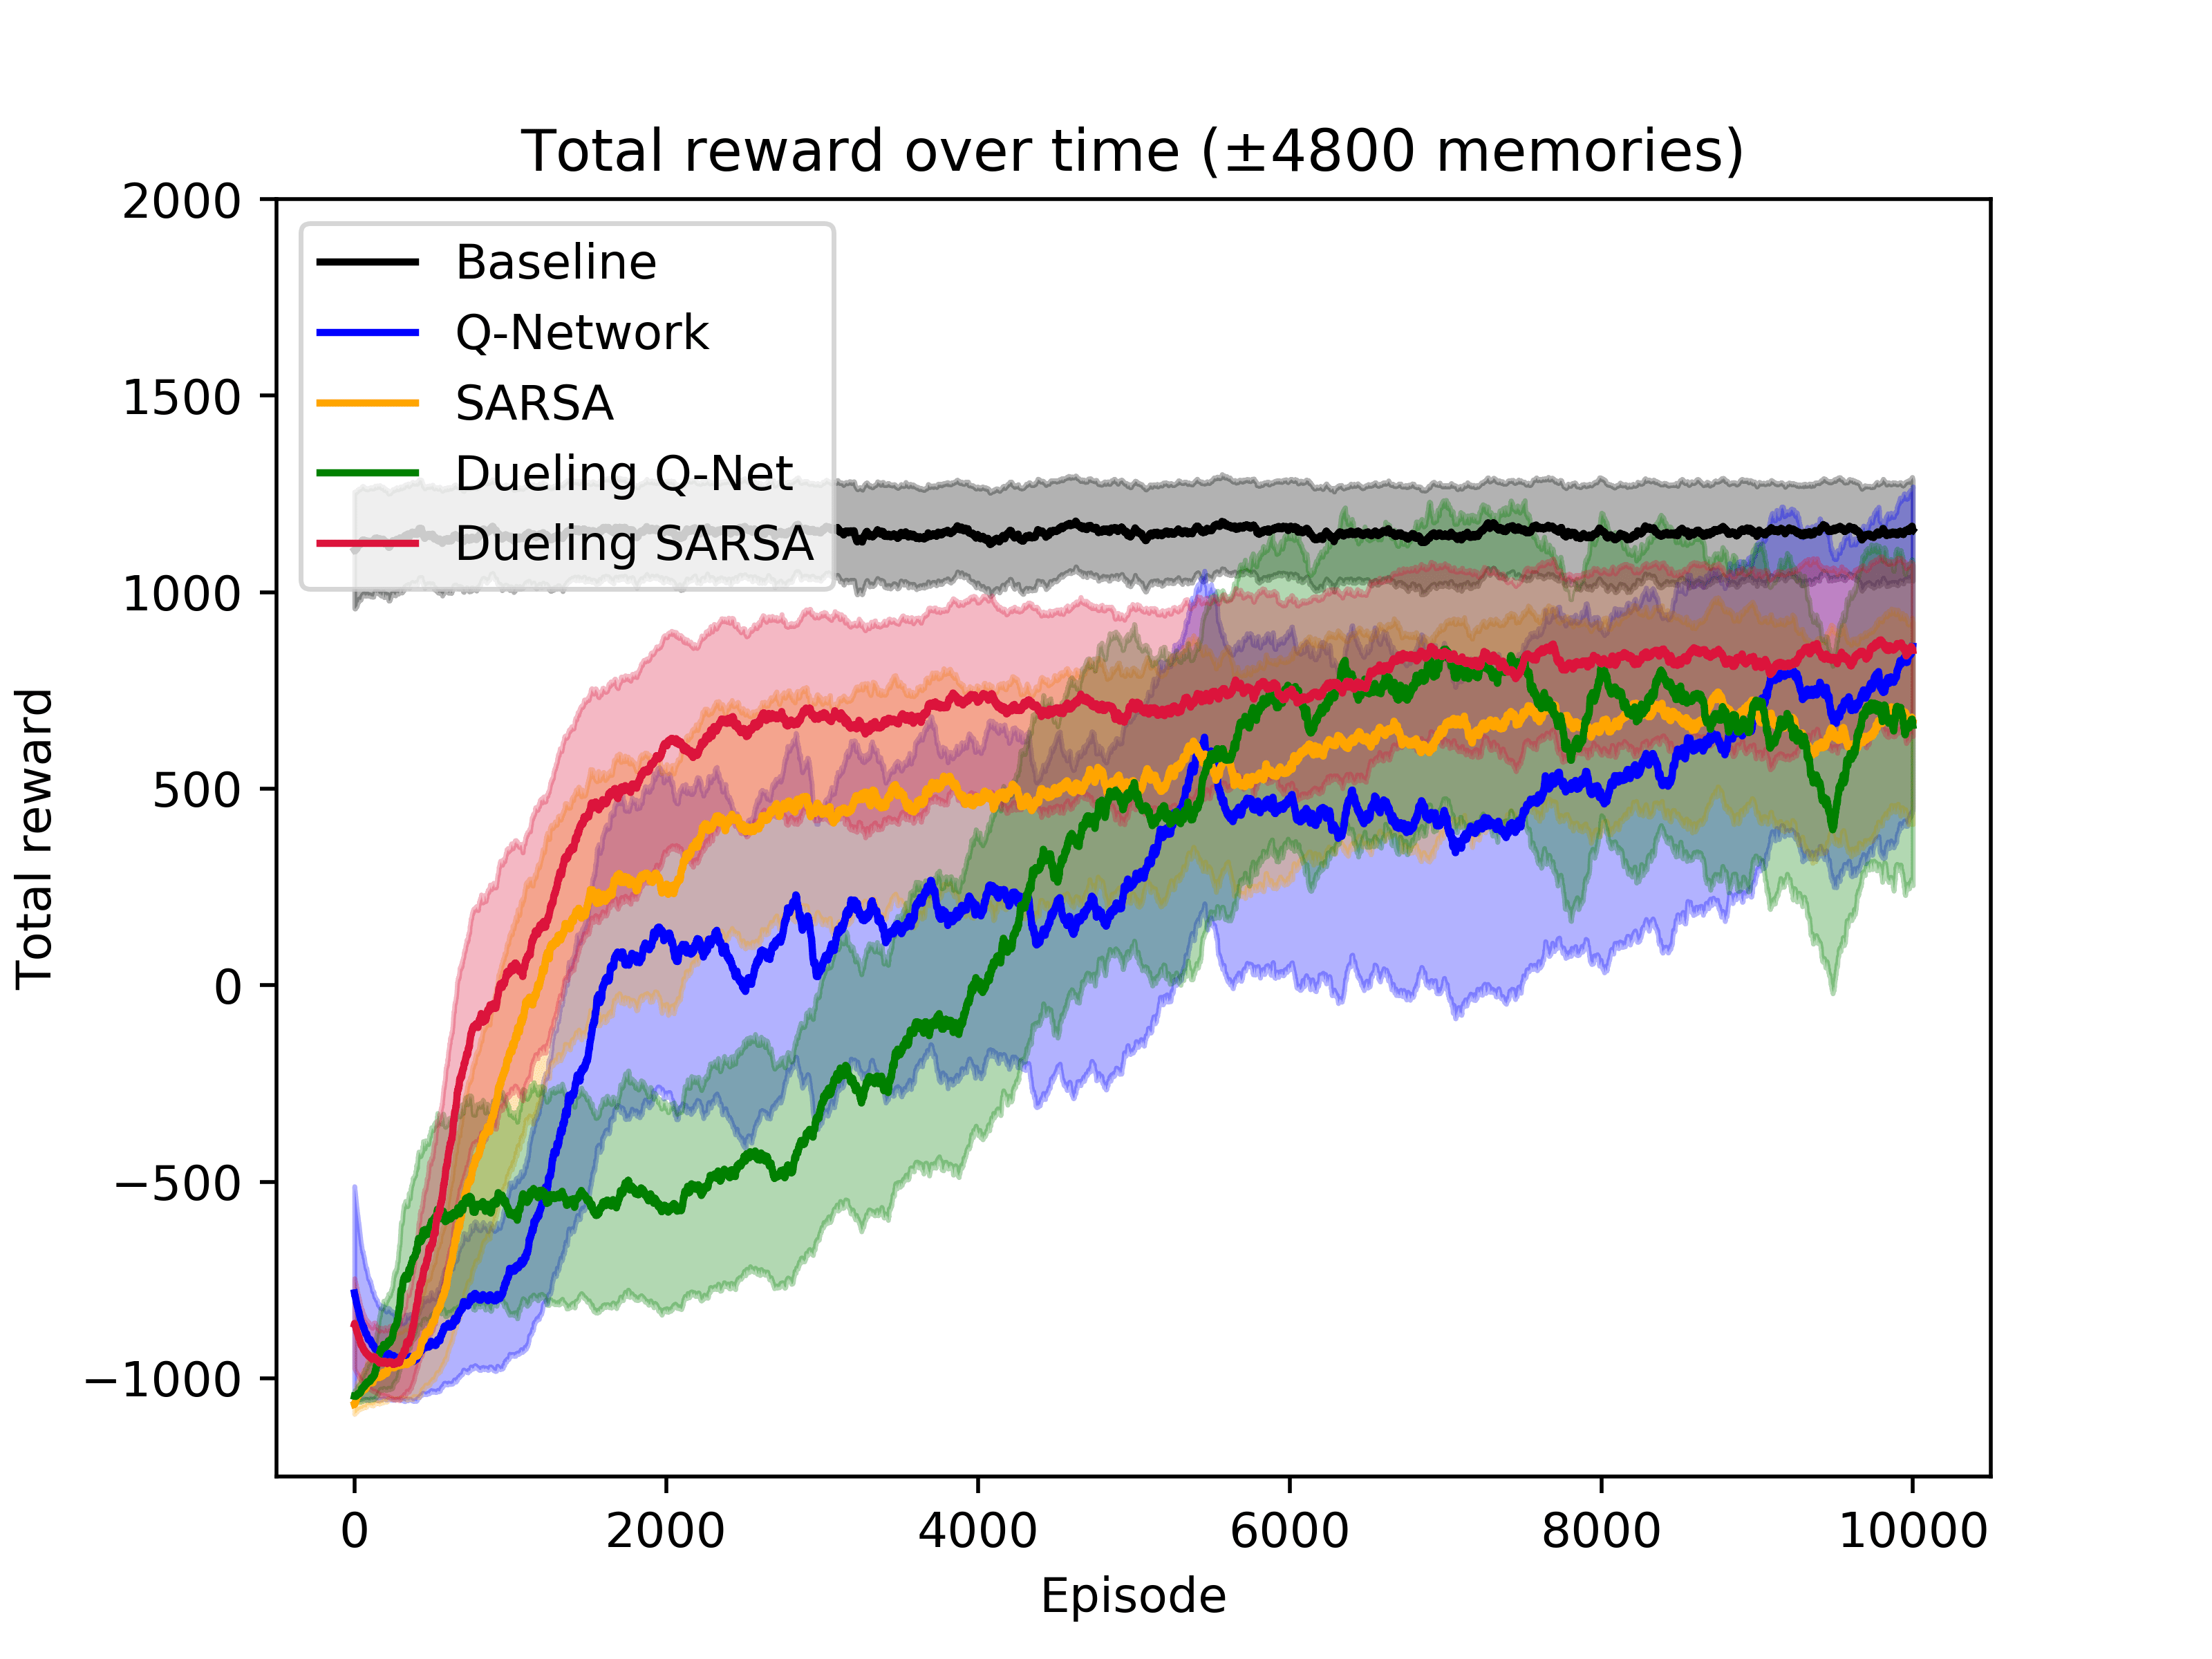
\includegraphics[width=\linewidth]{img/results/14-sized/total_rewards_100m-min.png}
    \caption{14-by-14 grid given 100 episodes of demonstation data.}
    \label{fig:14sized-100mem}
    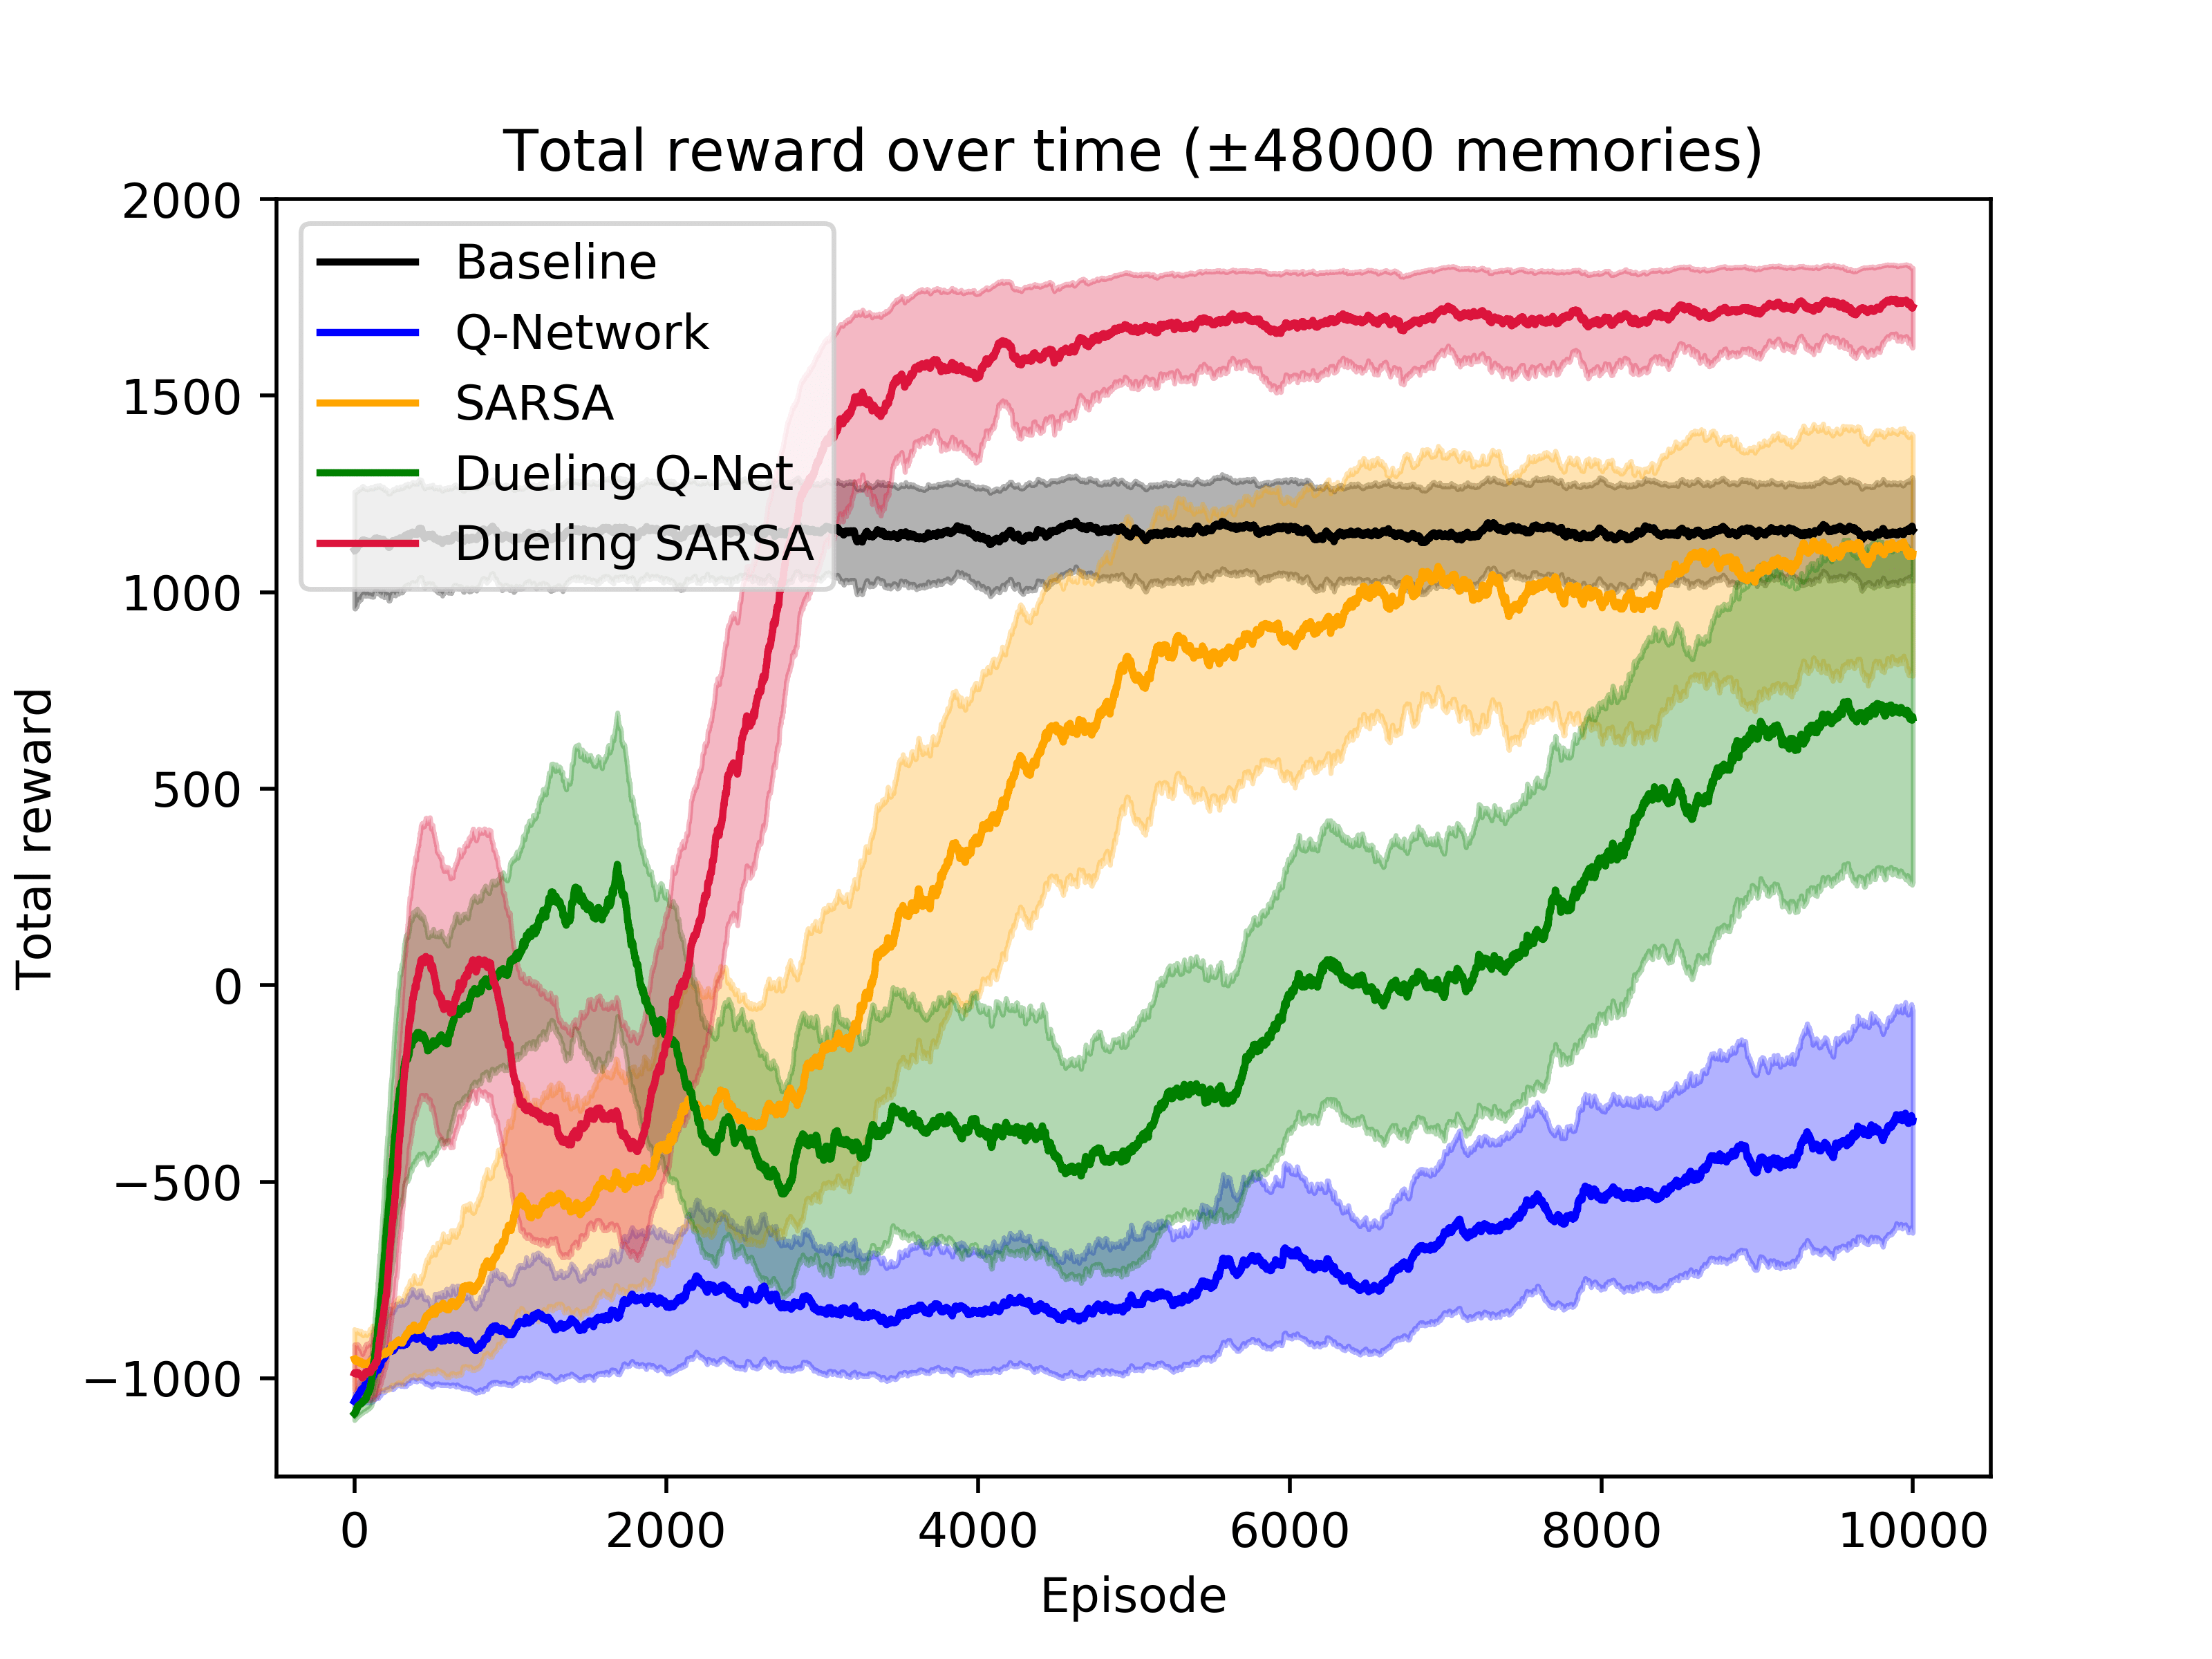
\includegraphics[width=\linewidth]{img/results/14-sized/total_rewards_1000m-min.png}
    \caption{14-by-14 grid given 1000 episodes of demonstation data.}
    \label{fig:14sized-1000mem}
\end{figure}